% Main chapter title
\chapter{Method of App Analysis}
\label{ch:dl}

% This is for the header on each page
\lhead{Chapter 4. \emph{Method of App Analysis}}
\thispagestyle{empty}
In Google Play Store, there are lots of malicious applications. So, we have tried to find the behaviour of application and restrict its malicious intent if any. In section 4.1, we have discussed our approach. In section 4.2, we have discussed about analysis of some applications.
\section{Design Approach}
There are nearly 3.6 million applications on Google play store \cite{availableapp}. Not all the applications are benign on the Google play store. Some applications may have security issues. Android also supports installation of application from third and third party application can not be trusted. So, we have proposed a mechanism to determine the behaviour of application. If we find behaviour of application as malicious, then we have to restrict the malicious behaviour of applications. We are doing the whole process in following three phases:
\begin{enumerate}
    \item Analysis of application.
    \item Determining behaviour of application.
    \item Restricting malicious intent of application.
\end{enumerate}
\begin{figure}[!h]
  \centering
  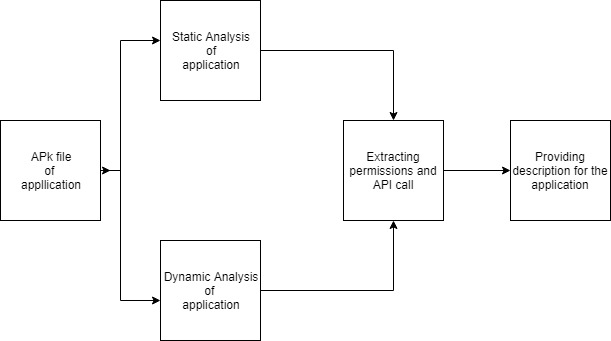
\includegraphics [scale=0.6] {archwork1.jpg}
  \caption{Workflow of analysis phase}
  \label{fig:archwork1}
\end{figure}

We are doing static and dynamic analysis of applications. For analyzing the application we are using Droidmate \cite{jamrozik2016droidmate}, RiskIndroid \cite{merlo2017riskindroid} and AndroPyTool \cite{andropytoool}. From the analysis we are extracting the permissions and API calls from the applications. After seeing the permissions required by applications and API calls it is invoking, we are proposing the description of the application. Workflow for analysis phase is shown in Figure \ref{fig:archwork1}.

\\
Using the analyzed data of applications whose class is known ( it is known that whether application is benign or malicious), we are developing the classification model with the help of various machine learning techniques such as Logistic Regression, Support Vector Machine, Neural Network and Random Forest. Once the model is built, we are using that classification model to determine the class of applications that we have analyzed. Workflow for classification phase is shown in Figure \ref{fig:archwork2}
\begin{figure}[!h]
  \centering
  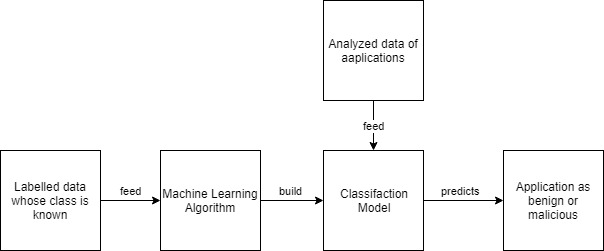
\includegraphics [scale=0.6] {archwork2.jpg}
  \caption{Workflow of classification phase}
  \label{fig:archwork2}
\end{figure}

Once we know that whether applications are malicious or benign, then we only focus of malicious applications. We try to restrict the malicious behaviour or intent of the applications by using a wrapper around the applications. Figure \ref{fig:archwork3} shows the workflow of restriction phase.

\begin{figure}[!h]
  \centering
  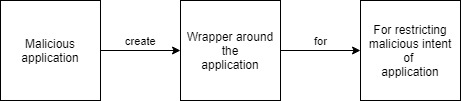
\includegraphics [scale=0.6] {archwork3.jpg}
  \caption{Workflow of restirction phase}
  \label{fig:archwork3}
\end{figure}




%---------------------------------------------------------------------%
\section{Analysis of Application}
In dynamic analysis, we are extracting several information like Unique APIs found, actionable views seen, unique API+event pairs found, and actionable unique views clicked. We trace the API calls that have been invoked while triggering UI elements. In static analysis, we are extracting information about permissions declared and used in application.

For dynamic analysis, we have used DROIDMATE which is fully automatic test generator for Android application and for static analysis we have used RiskInDroid which is python tool used for reverse engineering, malware and goodware analysis of Android application. We have also used AndoPyTool for both Dynamic and static analysis of applications.
\subsection{Budget Planner}
Budget Planner is an Android application which is used for managing your savings and expenses. Figure \ref{fig:bp} shows the screenshot taken during static analysis and Figure \ref{fig:bp1}  shows the screenshot taken during dynamic analysis of application.
\begin{figure}[!h]
  \centering
  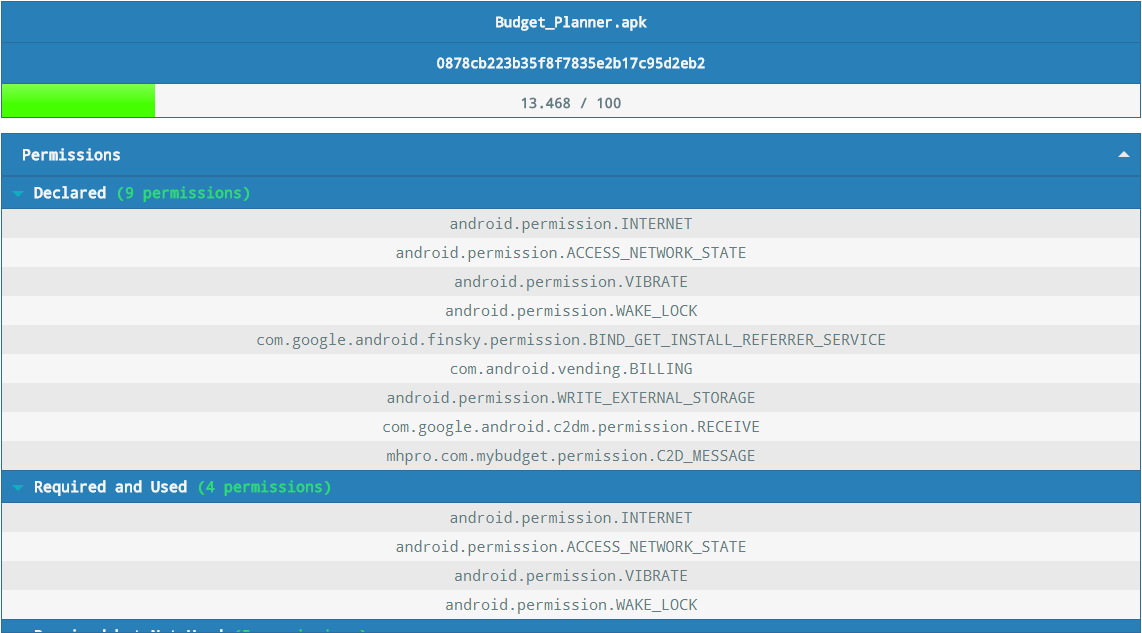
\includegraphics [scale=0.5] {bp.png}
  \caption{Screenshot captured during static analysis of Budget Planner app}
  \label{fig:bp}
\end{figure}
\subsubsection{Permissions}
We have extracted the following 9 permissions during the static analysis of Budget Planner app:\\
\textbf{Required and used} (4 permissions)
\begin{itemize}
    \begin{spacing}{0.9}
    \item \texttt{android.permission.INTERNET} \hfill - Dangerous
    \item \texttt{android.permission.ACCESS\_NETWORK\_STATE} \hfill - Dangerous
    \item \texttt{android.permission.VIBRATE}
    \item \texttt{android.permission.WAKE\_LOCK}
    \end{spacing}
\end{itemize}
\textbf{Required but not used} (5 permissions)
\begin{itemize}
    \begin{spacing}{0.9}
    \item \texttt{com.google.android.finsky.permission.BIND\_GET\_INSTALL\_REFERRER\_SERVICE}
    \item \texttt{com.android.vending.BILLING}
    \item \texttt{android.permission.WRITE\_EXTERNAL\_STORAGE} \hfill - Dangerous
    \item \texttt{com.google.android.c2dm.permission.RECEIVE}
    \item \texttt{mhpro.com.mybudget.permission.C2D\_MESSAGE}
    \end{spacing}
\end{itemize}
\begin{figure}[h]
	\centering
	\begin{subfigure}[h]{0.45\textwidth}
		\centering
		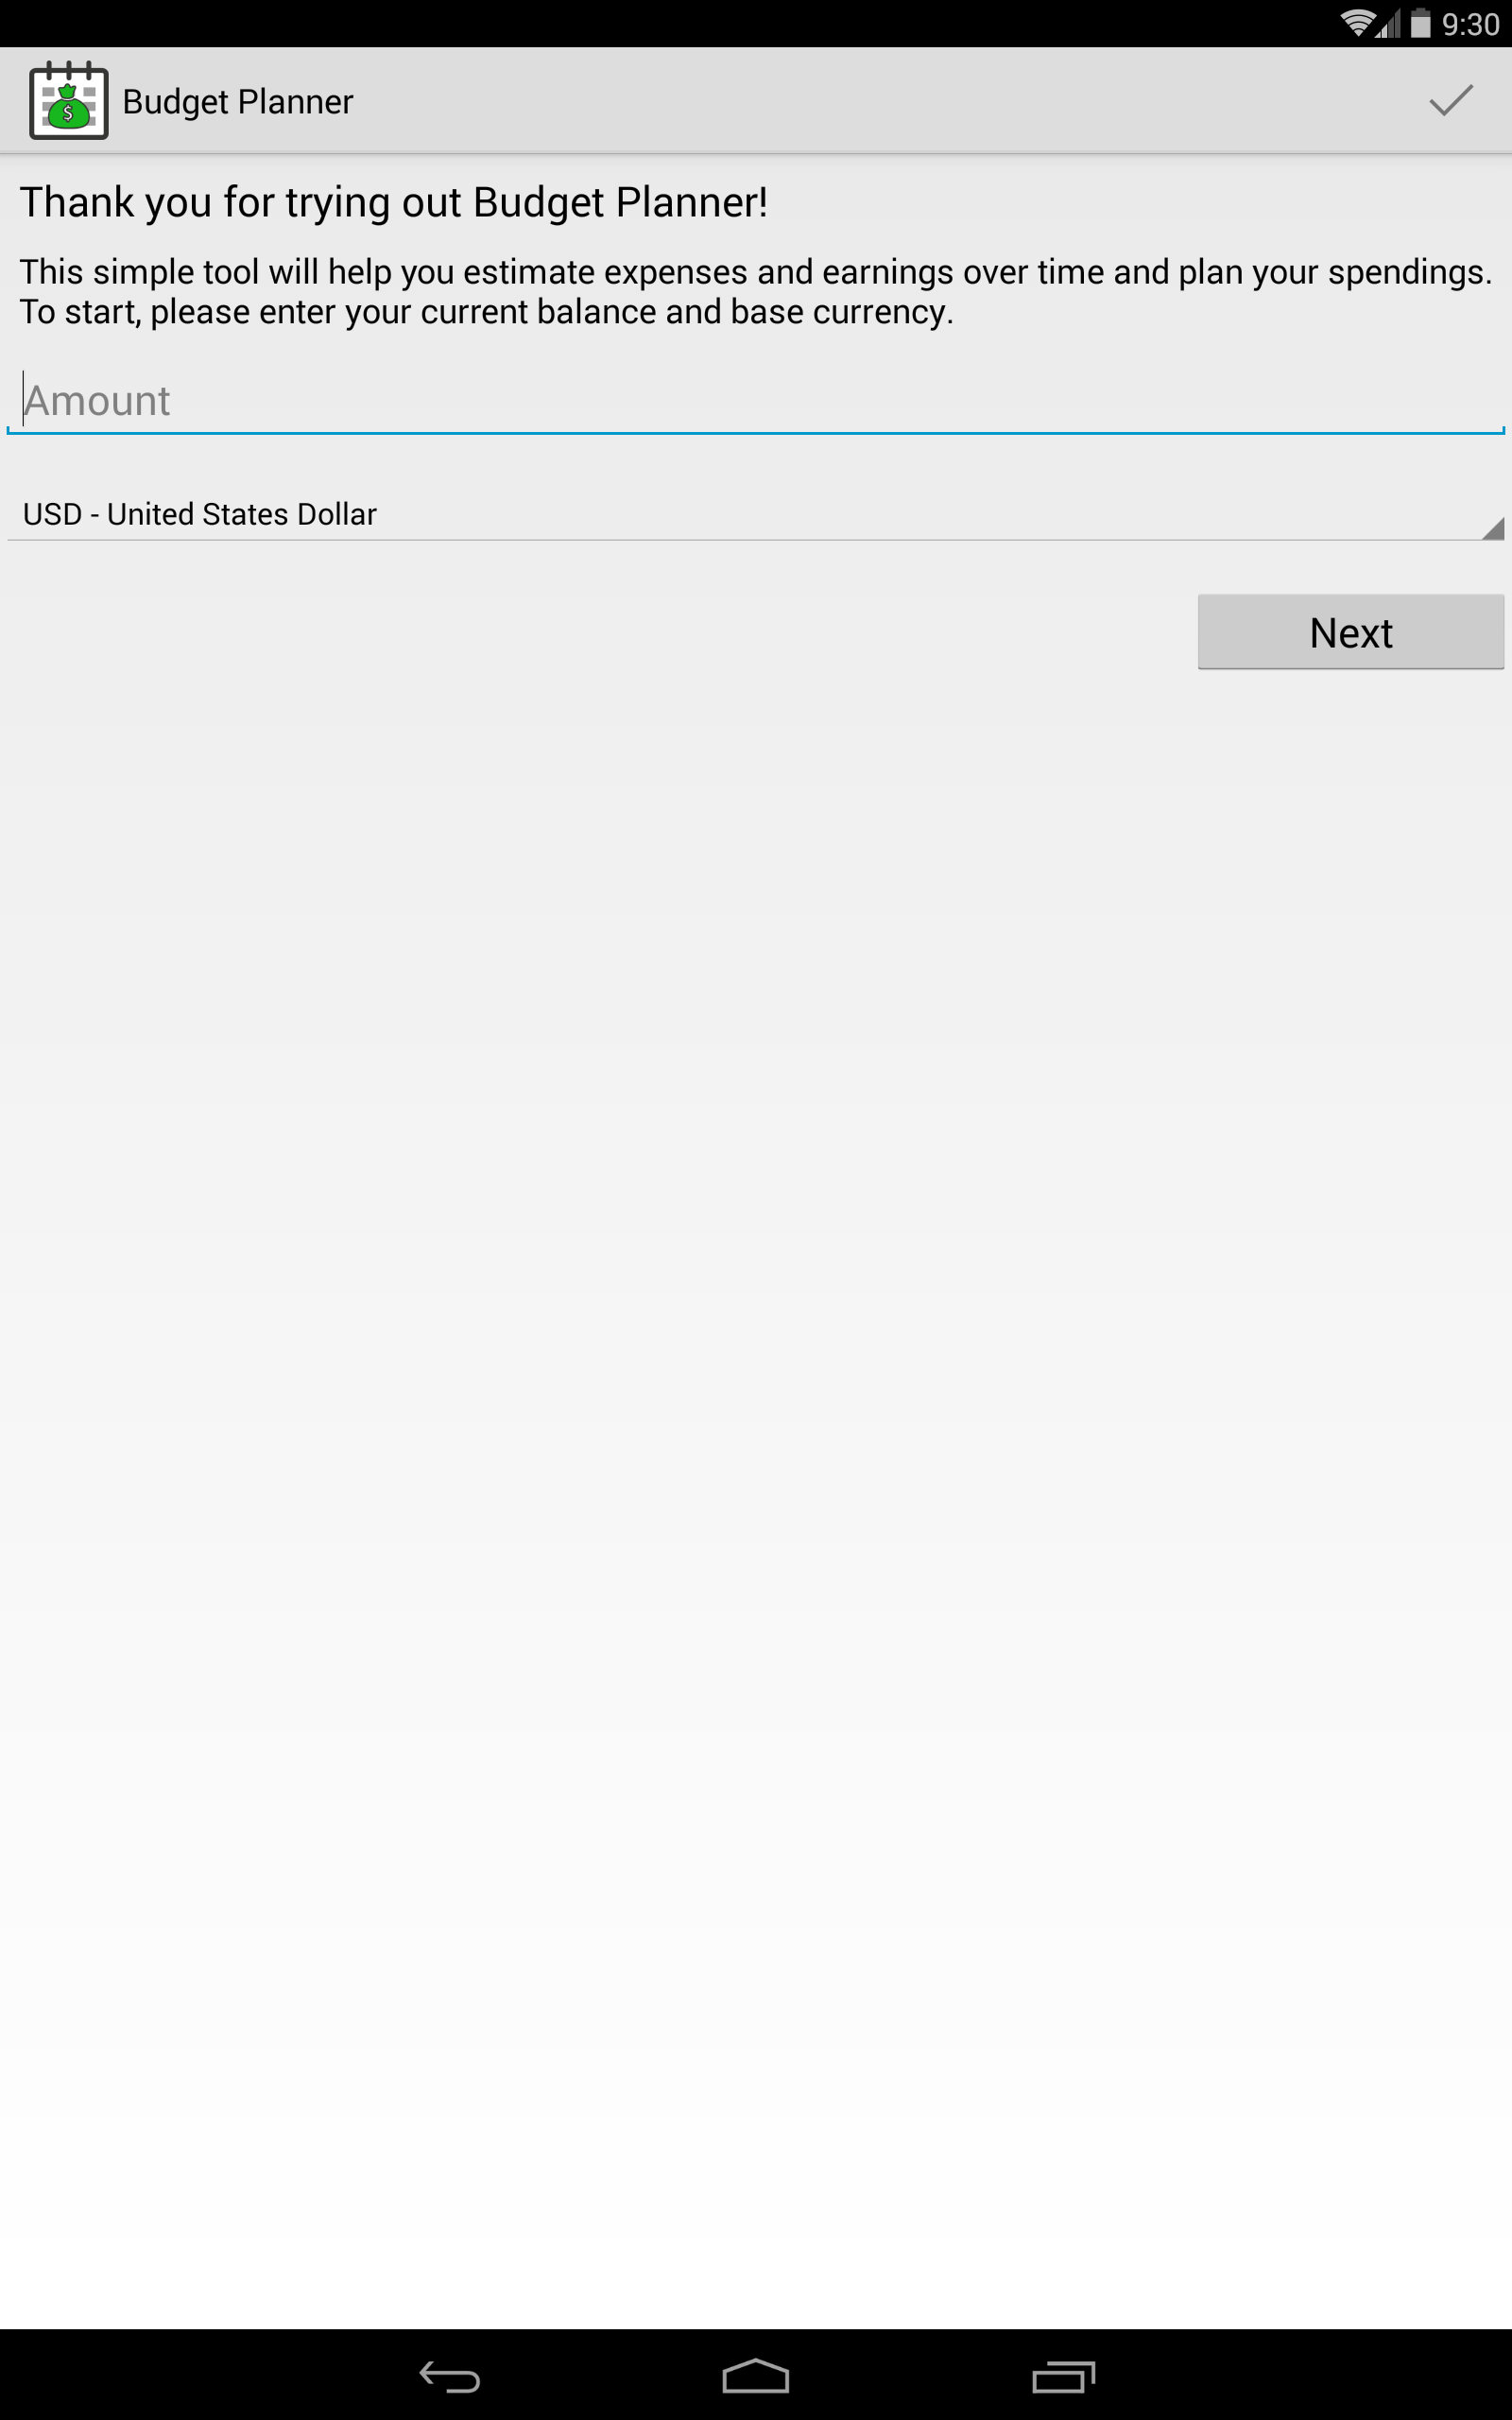
\includegraphics[width=\textwidth]{bp1.png}
		\caption{Budget Planner screenshot-1}
	\end{subfigure}
	\hfill
	\begin{subfigure}[h]{0.45\textwidth}
		\centering
		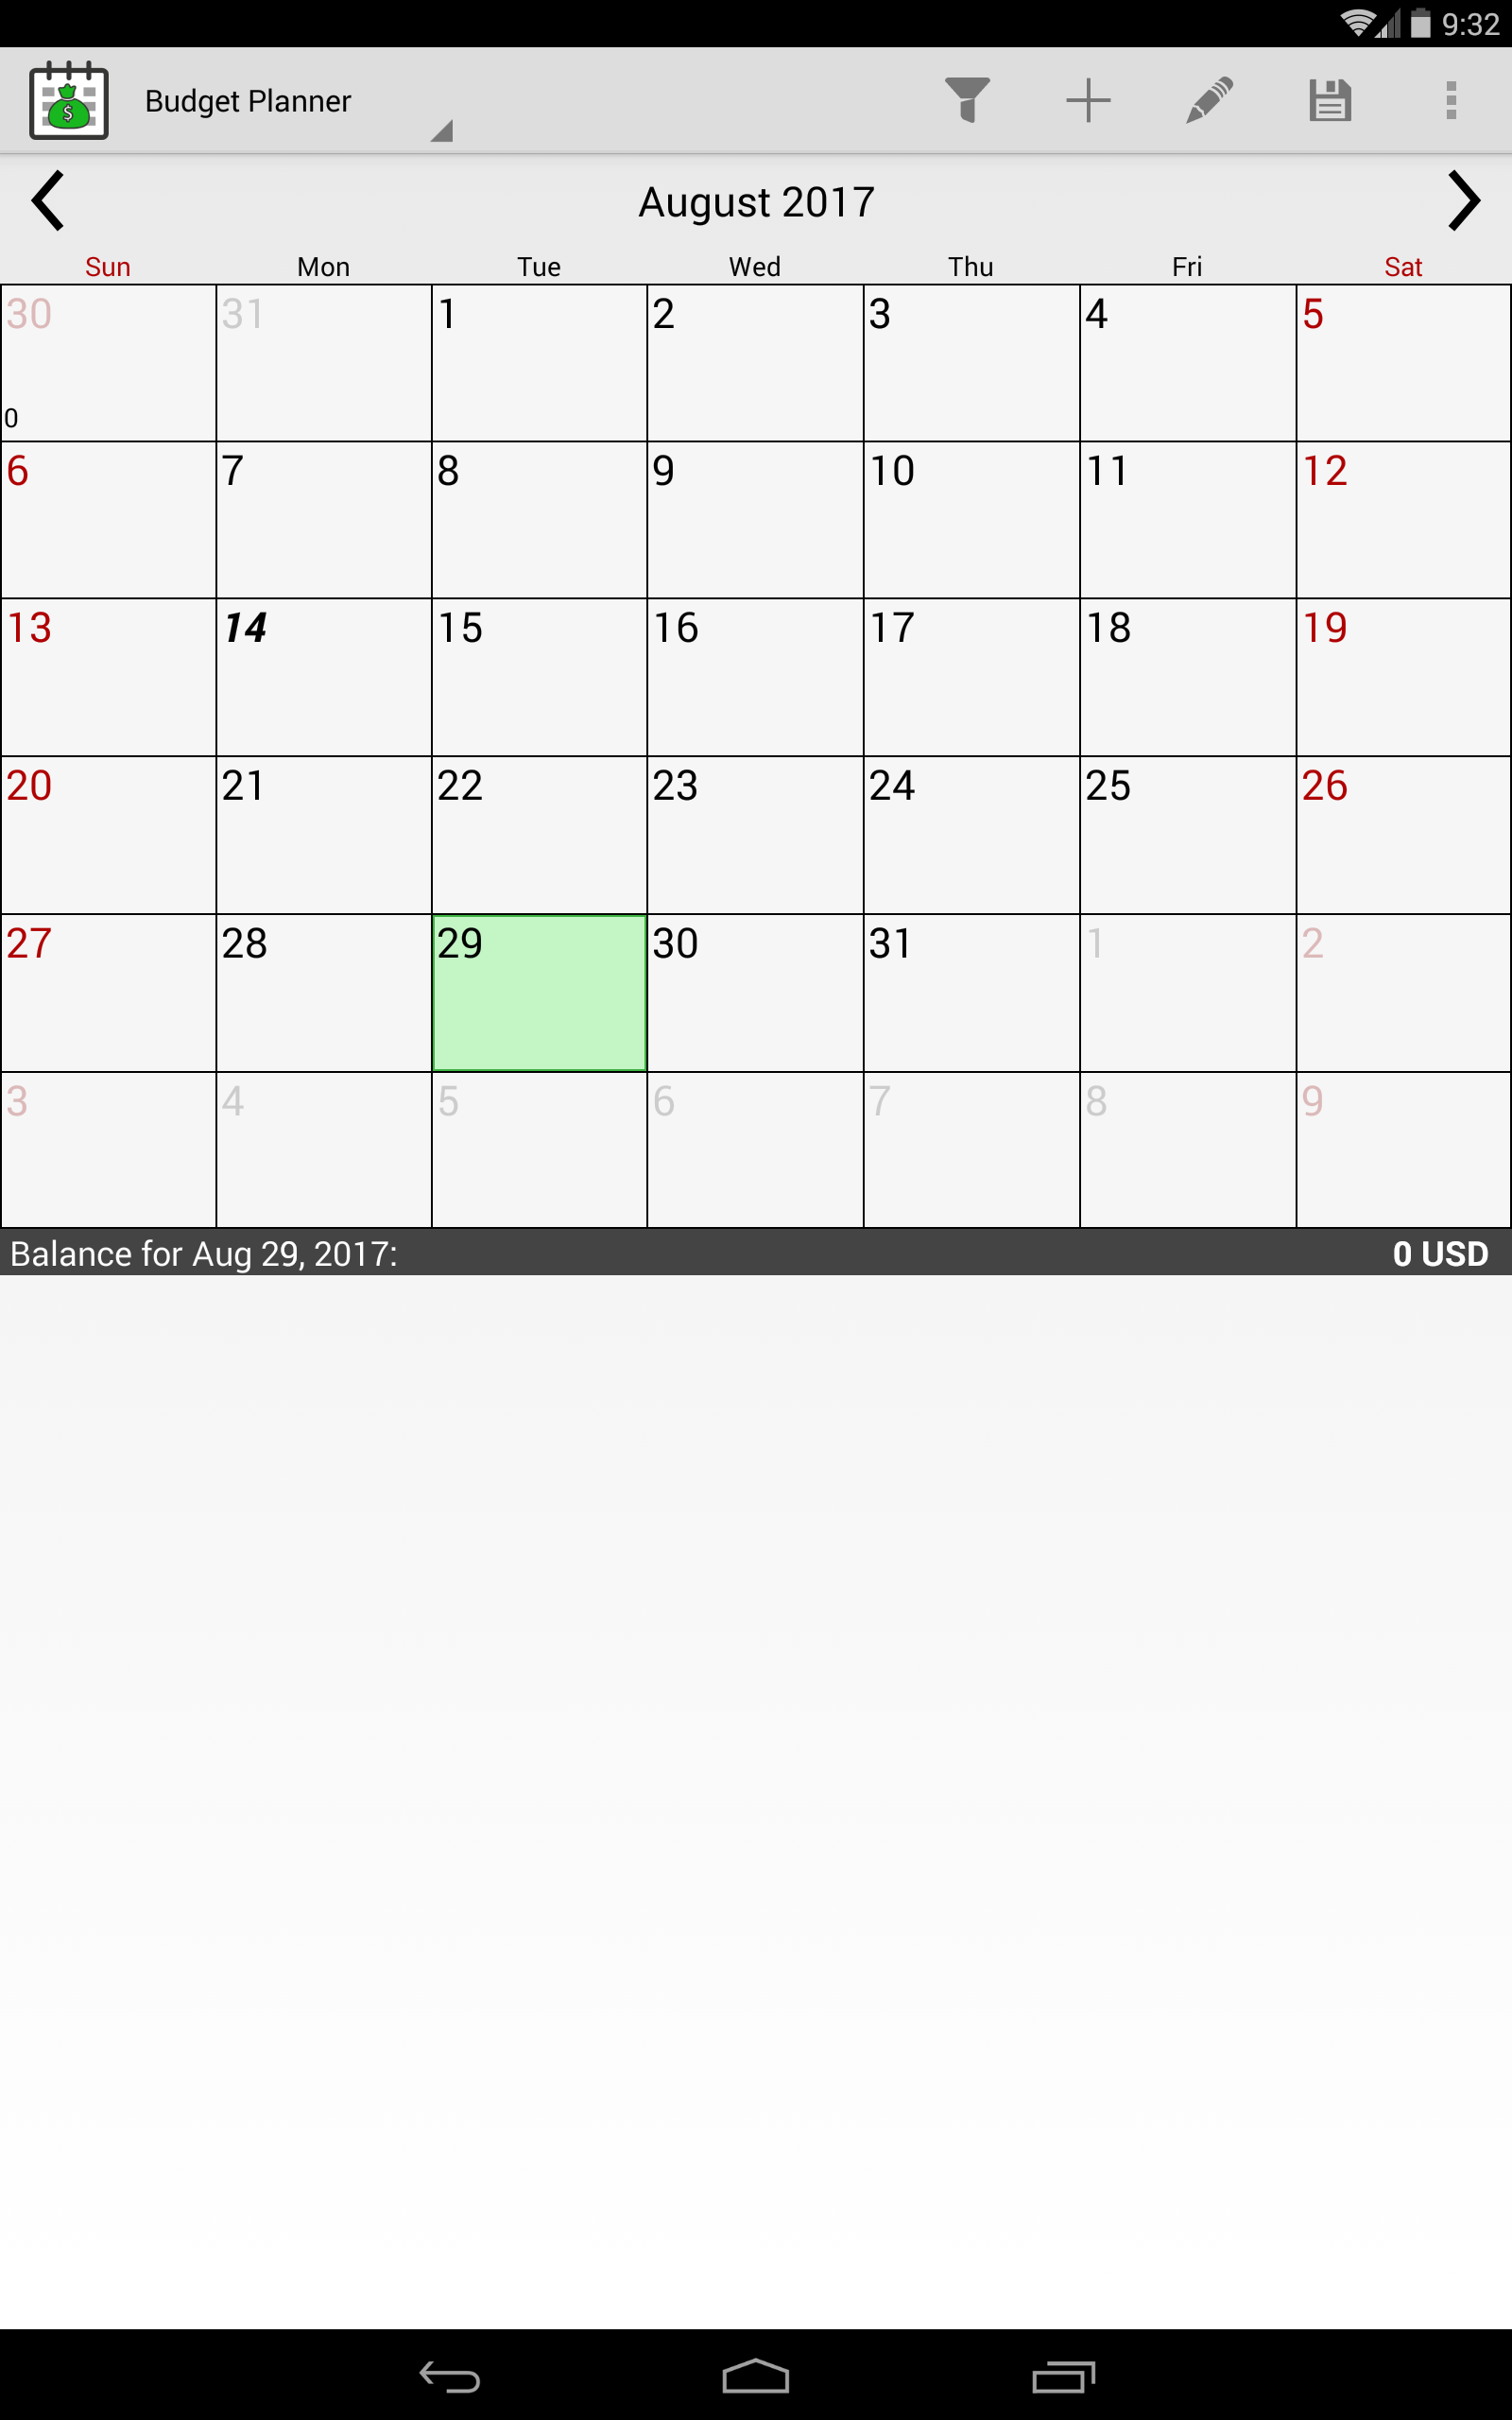
\includegraphics[width=\textwidth]{bp2.png}
		\caption{Budget Planner screenshot-2}
	\end{subfigure}
	\caption{Screenshot captured during analysis}
	\label{fig:bp1}
\end{figure}
\subsubsection{Unique Android SDK API methods}
Number of unique API calls count observed in the run is 4. Following is list of first calls to unique Android SDK API methods:
\begin{itemize}
    \item \texttt{0m 12s - android.telephony.TelephonyManager: java.lang.String getDeviceId()}
\item \texttt{0m 12s - org.apache.http.impl.client.AbstractHttpClient: org.apache.http. HttpResponse (org.apache.http.HttpHost, org.apache.http.protocol.HttpContext)}
\item \texttt{0m 13s - java.net.Socket: void connect (java.net.SocketAddress,int)}
 \item \texttt{0m 13s - android.location.LocationManager: java.lang.String getBestProvider (android.location.Criteria,boolean)}

\end{itemize}
\subsubsection{Unique [API call, event] Android SDK API methods}
Number of unique [API call, event] pairs count observed in the run is 5. Following is the list of first calls to unique Android SDK API methods:
\begin{itemize}
    \item \texttt{0m 12s - reset - android.telephony.TelephonyManager: java.lang.String getDeviceId()}
\item \texttt{0m 12s -  reset - org.apache.http.impl.client.AbstractHttpClient: org.apache. HttpResponse (org.apache.http.HttpHost, org.apache.http.protocol.HttpContext)}
\item \texttt{0m 13s -  reset - java.net.Socket: void connect (java.net.SocketAddress,int)}
\item \texttt{0m 13s -  reset - android.location.LocationManager: java.lang.String.get. BestProvider (android.location.Criteria,boolean)}
\item \texttt{2m 17s - background - android.location.LocationManager:java.lang.String. getBestProvider\\(android.location.Criteria,boolean)}

\end{itemize}
\\
\newline
Figure \ref{fig:bp3} shows the time at which different APIs and (API call, event) pairs are discovered. Total API discovered is 4 and total (API call,event) pair discoverd is 5.
\begin{figure}[!h]
  \centering
  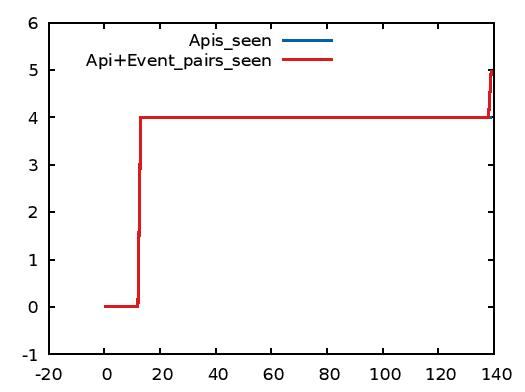
\includegraphics [scale=1.4] {bp3.jpg}
  \caption{API count vs Exploration time}
  \label{fig:bp3}
\end{figure}

\subsubsection{Actionable views}
According Figure \ref{fig:bp4}, nearly 180 unique actionable views is seen and 33 out of 180 views are clicked. The Table \ref{table:1} shows 32 views are clicked once and one views are clicked thrice. 
\begin{figure}[!h]
  \centering
  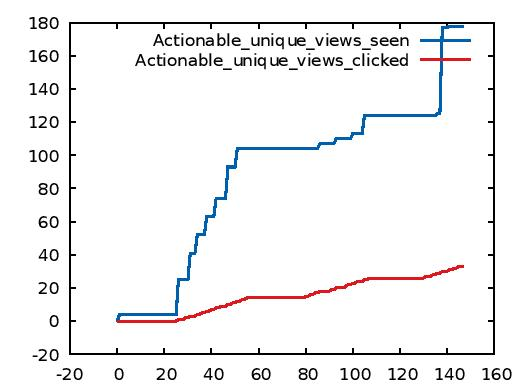
\includegraphics [scale=1.4] {bp4.jpg}
  \caption{API count vs Exploration time}
  \label{fig:bp4}
\end{figure}

\begin{table}[h!]
\centering
\begin{tabular}{||c | c||} 
 \hline
 Number of Click & Views Count \\ [0.5ex] 
 \hline\hline
 0 & 0 \\ 
 1 & 32\\
 2 & 0 \\
 3 & 1\\ [1ex] 

 \hline
\end{tabular}
\caption{Click Frequency of views}

\label{table:1}
\end{table}

\subsubsection{Aggregate stats}
Following is the summary of dynamic analysis of Budget planner application:
\begin{itemize}
    \item File name - budget\_planner-inlined.apk
\item Package name - bdget\_planner
\item Exploration seconds - 153
\item Actions - 39
\item In this reset actions - 3
\item Actionable unique views seen at least once - 178
\item Actionable unique views clicked or long clicked at least once - 33
\item Unique apis - 4
\item Unique event api pairs - 5
\item Exception - N/A (lack of DeviceException)

\end{itemize}

%---------------------------------------------------------------------%
\subsection{BHIM Making India Cashless}
Bharat Interface for Money (BHIM) is an initiative to enable fast, secure, reliable cashless payments through your mobile phone. BHIM is inter operable with other Unified Payment Interface (UPI) applications, & bank accounts for quick money transfers online.
Figure \ref{fig:bhim} shows screenshot taken during the analysis of BHIM applications.
\begin{figure}[!h]
  \centering
  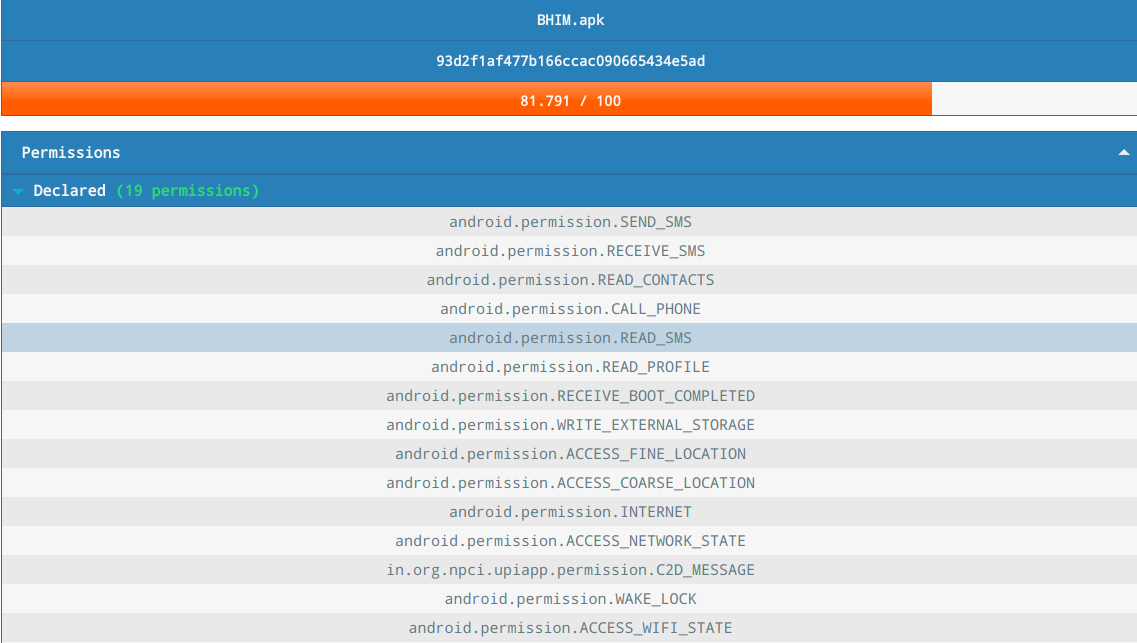
\includegraphics [scale=0.5] {bhim.png}
  \caption{Screenshot captured during analysis of BHIM app}
  \label{fig:bhim}
\end{figure}
\subsubsection{Permissions}
We have extracted the following permissions during the static analysis of BHIM app:\\
\textbf{Required and used} (6 permissions)
\begin{itemize}
    \begin{spacing}{0.9}
    \item \texttt{android.permission.ACCESS\_FINE\_LOCATION} \hfill - Dangerous
    \item \texttt{android.permission.ACCESS\_COARSE\_LOCATION} \hfill - Dangerous
    \item \texttt{android.permission.INTERNET}
    \item \texttt{android.permission.ACCESS\_NETWORK\_STATE}
    \item \texttt{android.permission.WAKE\_LOCK}
    \item \texttt{android.permission.READ\_PHONE\_STATE} \hfill - Dangerous
    \end{spacing}
\end{itemize}
\textbf{Required but not used}(13 permissions)
\begin{itemize}
    \begin{spacing}{0.9}
    \item \texttt{android.permission.SEND\_SMS} \hfill - Dangerous
    \item \texttt{android.permission.RECEIVE\_SMS} \hfill - Dangerous
    \item \texttt{android.permission.READ\_CONTACTS} \hfill - Dangerous
    \item \texttt{android.permission.CALL\_PHONE} \hfill - Dangerous
    \item \texttt{android.permission.READ\_SMS} \hfill - Dangerous
    \item \texttt{android.permission.READ\_PROFILE}
    \item \texttt{android.permission.RECEIVE\_BOOT\_COMPLETED}
    \item \texttt{android.permission.WRITE\_EXTERNAL\_STORAGE} \hfill - Dangerous
    \item \texttt{in.org.npci.upiapp.permission.C2D\_MESSAGE}
    \item \texttt{android.permission.ACCESS\_WIFI\_STATE}
    \item \texttt{android.permission.CAMERA} \hfill - Dangerous
    \item \texttt{android.permission.READ\_EXTERNAL\_STORAGE} \hfill - Dangerous
    \item \texttt{com.google.android.c2dm.permission.RECEIVE}
    \end{spacing}
\end{itemize}
\textbf{Not required but used}(1 permissions)
\begin{itemize}
    \item \texttt{android.permission.VIBRATE}
\end{itemize}

\subsection{Funnyys}
Funnyys is an application which can add charges to your mobile bill by sending costly SMS messages without informing you first. Figure \ref{fig:funnyys} shows screenshot taken during analysis Funnyys app.
\begin{figure}[!h]
  \centering
  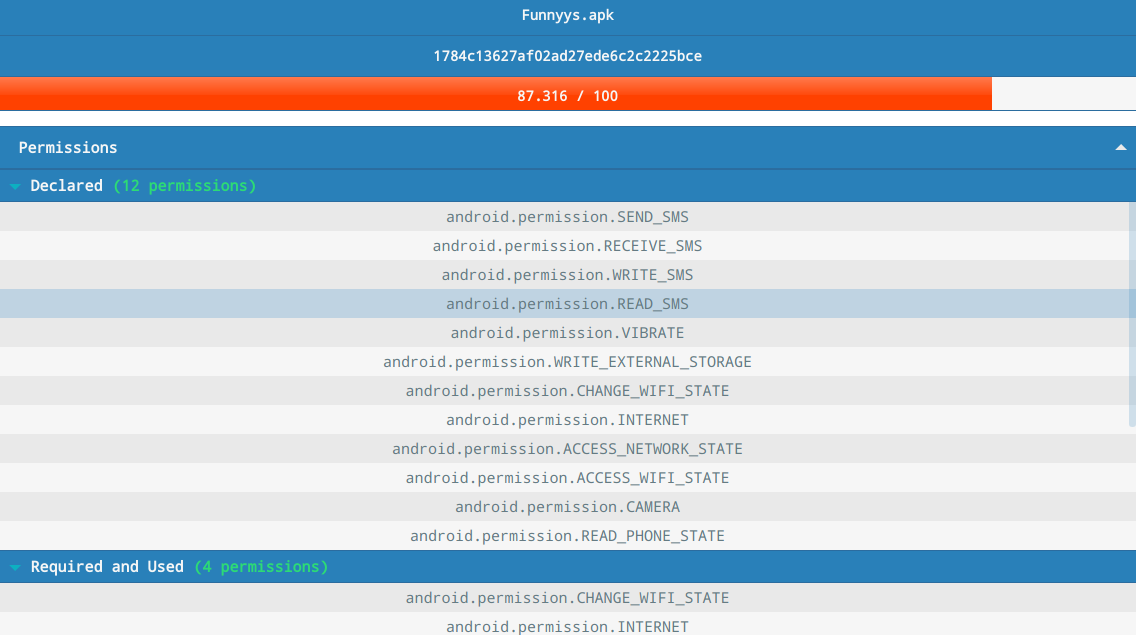
\includegraphics [scale=0.5] {funnyys.png}
  \caption{Screenshot captured during analysis of Funnyys app}
  \label{fig:funnyys}
\end{figure}
\subsubsection{Permissions}
We have extracted the following permissions during the static analysis of Funnyys app:\\
\textbf{Required and used} (4 permissions)
\begin{itemize}
\begin{spacing}{0.9}
\item \texttt{android.permission.CHANGE\_WIFI\_STATE}
\item \texttt{android.permission.INTERNET}
\item \texttt{android.permission.ACCESS\_NETWORK\_STATE}
\item \texttt{android.permission.ACCESS\_WIFI\_STATE}
\end{spacing}
\end{itemize}
\textbf{Required but not used} (8 permissions)
\begin{itemize}
\begin{spacing}{0.9}
\item \texttt{android.permission.SEND\_SMS} \hfill - Dangerous
\item \texttt{android.permission.RECEIVE\_SMS} \hfill - Dangerous
\item \texttt{android.permission.WRITE\_SMS} \hfill - Dangerous
\item \texttt{android.permission.READ\_SMS} \hfill - Dangerous
\item \texttt{android.permission.VIBRATE}
\item \texttt{android.permission.WRITE\_EXTERNAL\_STORAGE} \hfill - Dangerous
\item \texttt{android.permission.CAMERA} \hfill - Dangerous
\item \texttt{android.permission.READ\_PHONE\_STATE} \hfill - Dangerous
\end{spacing}
\end{itemize}
\textbf{Not required but used}(1 permission)
\begin{itemize}
    \item \texttt{android.permission.WAKE\_LOCK}
\end{itemize}
\subsection{Omingo}
This app lets hackers control your device, giving them unauthorized access to your data. Figure \ref{fig:omingo} shows screenshot taken during analysis of Omingo app.
\begin{figure}[!h]
  \centering
  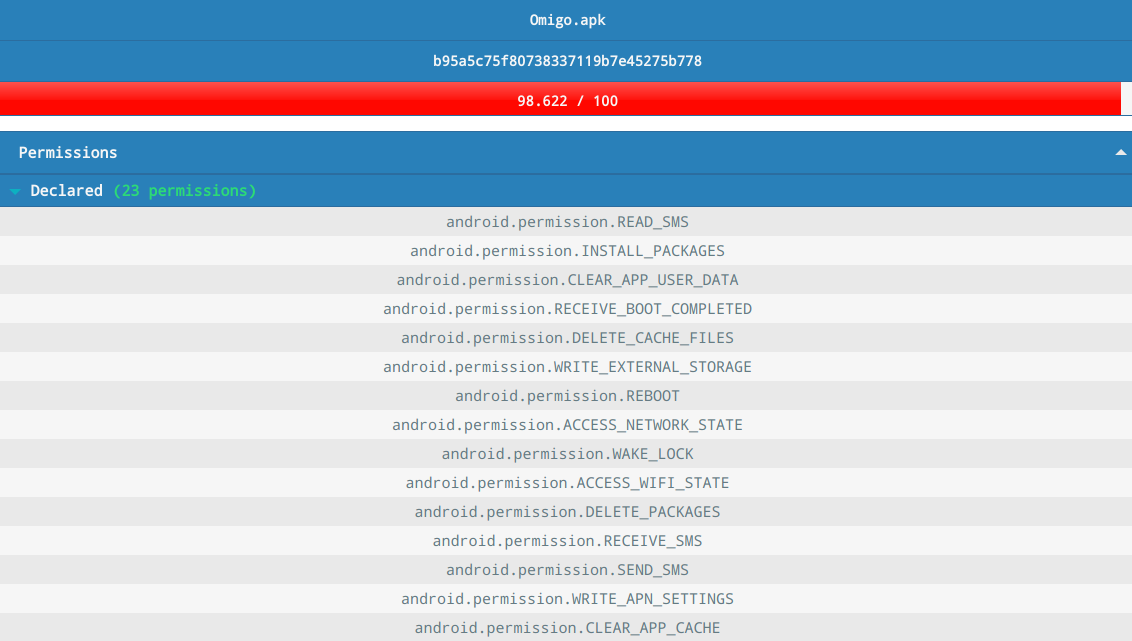
\includegraphics [scale=0.5] {omigo.png}
  \caption{Screenshot captured during analysis of Omingo app}
  \label{fig:omingo}
\end{figure}
\subsubsection{Permissions}
We have extracted the following permissions during the static analysis of Omingo app:\\
\textbf{Required and used} (4 permissions)
\begin{itemize}
\begin{spacing}{0.9}
\item \texttt{android.permission.INTERNET}
\item \texttt{android.permission.ACCESS\_NETWORK\_STATE}
\item \texttt{android.permission.ACCESS\_WIFI\_STATE}
\item \texttt{android.permission.READ\_PHONE\_STATE} \hfill - Dangerous
\end{spacing}
\end{itemize}
\textbf{Required but not used} (19 permissions)
\begin{itemize}
\begin{spacing}{0.9}
\item \texttt{android.permission.RECEIVE\_SMS} \hfill - Dangerous
\item \texttt{android.permission.SEND\_SMS} \hfill - Dangerous
\item \texttt{android.permission.WRITE\_APN\_SETTINGS}
\item \texttt{android.permission.CLEAR\_APP\_CACHE}
\item \texttt{android.permission.READ\_SMS} \hfill - Dangerous
\item \texttt{android.permission.RECEIVE\_WAP\_PUSH}
\item \texttt{android.permission.INSTALL\_PACKAGES} \hfill - Dangerous
\item \texttt{android.permission.CLEAR\_APP\_USER\_DATA}
\item \texttt{android.permission.MOUNT\_UNMOUNT\_FILESYSTEMS}
\item \texttt{android.permission.RECEIVE\_BOOT\_COMPLETED}
\item \texttt{android.permission.DELETE\_CACHE\_FILES}
\item \texttt{android.permission.WRITE\_EXTERNAL\_STORAGE} \hfill - Dangerous
\item \texttt{android.permission.REBOOT} \hfill - Dangerous
\item \texttt{android.permission.RESTART\_PACKAGES} \hfill - Dangerous
\item \texttt{android.permission.CHANGE\_WIFI\_STATE}
\item \texttt{android.permission.WAKE\_LOCK}
\item \texttt{android.permission.CHANGE\_NETWORK\_STATE}
\item \texttt{android.permission.SET\_WALLPAPER}
\item \texttt{android.permission.DELETE\_PACKAGES} \hfill - Dangerous
\end{spacing}
\end{itemize}
\textbf{Not required but used}(3 permission)
\begin{itemize}
\begin{spacing}{0.9}
\item \texttt{android.permission.ACCESS\_FINE\_LOCATION} \hfill - Dangerous
\item \texttt{android.permission.ACCESS\_COARSE\_LOCATION} \hfill - Dangerous
\item \texttt{android.permission.VIBRATE}
\end{spacing}
\end{itemize}
\subsection{System Certificate}
System Certificate  is a fake application which can damage your device and steal your data. Figure \ref{fig:system} shows the screenshot taken during static analysis of System Certificate app.
\begin{figure}[!h]
  \centering
  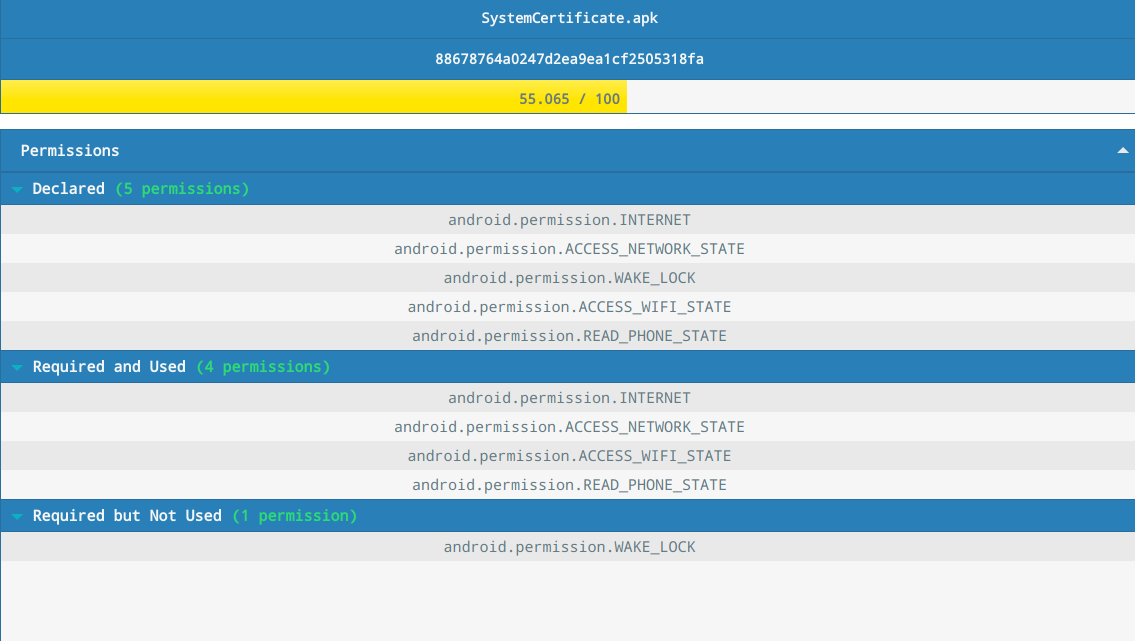
\includegraphics [scale=0.5] {system.png}
  \caption{Screenshot captured during analysis of System Certificate app}
  \label{fig:system}
\end{figure}
\subsubsection{Permissions}
We have extracted the following permissions during the static analysis of System Certificate app:\\

\textbf{Required and used} (4 permissions)
\begin{itemize}
\begin{spacing}{0.9}
\item \texttt{android.permission.INTERNET}
\item \texttt{android.permission.ACCESS\_NETWORK\_STATE}
\item \texttt{android.permission.ACCESS\_WIFI\_STATE}
\item \texttt{android.permission.READ\_PHONE\_STATE} \hfill - Dangerous
\end{spacing}
\end{itemize}
\textbf{Required but not used} (1 permissions)
\begin{itemize}
    \item \texttt{android.permission.WAKE\_LOCK}
\end{itemize}

\subsection{Tez – A new payments app by Google}
Tez is an application send money to others. It is developed by Google. It is based on UPI. Figure \ref{fig:tez} shows the screenshot taken during the analysis Tez app.
\begin{figure}[!h]
  \centering
  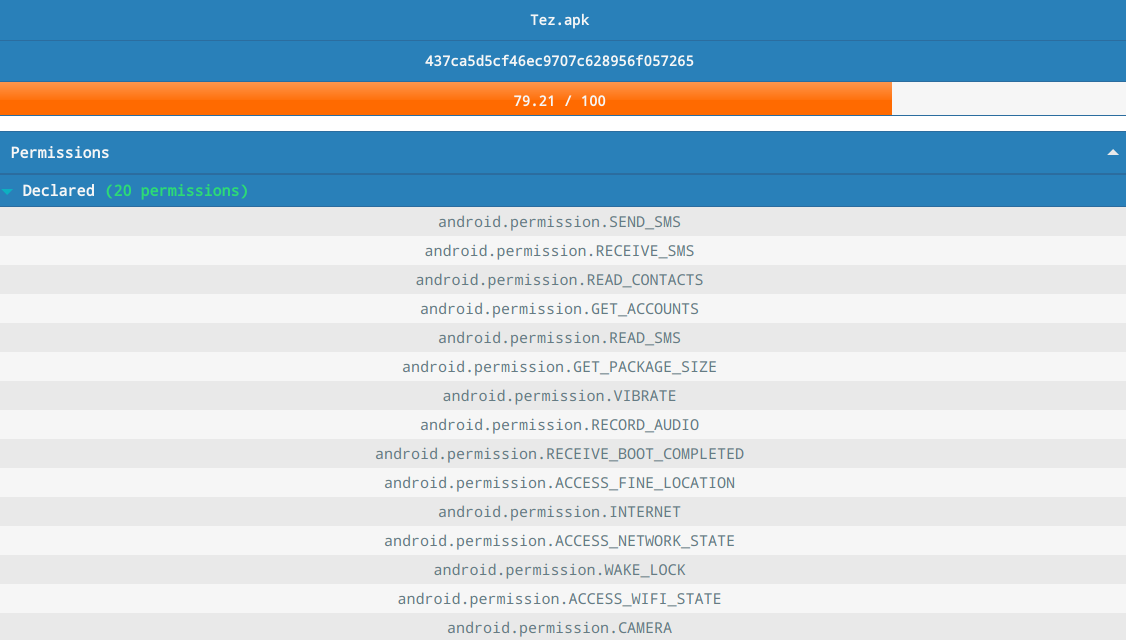
\includegraphics [scale=0.5] {tez.png}
  \caption{Screenshot captured during analysis of Tez app}
  \label{fig:tez}
\end{figure}
\subsubsection{Permissions}
We have extracted the following permissions during the static analysis of Tez app:\\
\textbf{Required and used} (6 permissions)
\begin{itemize}
\begin{spacing}{0.9}
\item \texttt{android.permission.INTERNET}
\item \texttt{android.permission.VIBRATE}
\item \texttt{android.permission.ACCESS\_NETWORK\_STATE}
\item \texttt{android.permission.WAKE\_LOCK}
\item \texttt{android.permission.BLUETOOTH}
\item \texttt{android.permission.READ\_PHONE\_STATE} \hfill - Dangerous
\end{spacing}
\end{itemize}
\textbf{Required but not used} (14 permissions)
\begin{itemize}
\begin{spacing}{0.9}
\item \texttt{android.permission.SEND\_SMS} \hfill - Dangerous
\item \texttt{android.permission.RECEIVE\_SMS} \hfill - Dangerous
\item \texttt{android.permission.READ\_CONTACTS} \hfill - Dangerous
\item \texttt{android.permission.GET\_ACCOUNTS} \hfill - Dangerous
\item \texttt{android.permission.READ\_SMS} \hfill - Dangerous
\item \texttt{android.permission.GET\_PACKAGE\_SIZE}
\item \texttt{android.permission.RECORD\_AUDIO} \hfill - Dangerous
\item \texttt{android.permission.RECEIVE\_BOOT\_COMPLETED}
\item \texttt{android.permission.ACCESS\_FINE\_LOCATION} \hfill - Dangerous
\item \texttt{android.permission.ACCESS\_WIFI\_STATE}
\item \texttt{android.permission.CAMERA} \hfill - Dangerous
\item \texttt{android.permission.MANAGE\_ACCOUNTS} \hfill - Dangerous
\item \texttt{com.google.android.c2dm.permission.RECEIVE}
\item \texttt{com.google.android.providers.gsf.permission.READ\_GSERVICES}
\end{spacing}
\end{itemize}
\textbf{Not required but used} (2 permission)
\begin{itemize}
\item \texttt{android.permission.ACCESS\_COARSE\_LOCATION} \hfill - Dangerous
\item \texttt{android.permission.MODIFY\_AUDIO\_SETTINGS}
\end{itemize}
\subsection{MMS Beline}
MMS Beline is an application which can call phone number  and also send SMS without informing you, which will lead to increase in mobile bill. This application can steal your data and can run with administrative permissions. Figure \ref{fig:mms} shows the screenshot taken during the static analysis of MMS Beline.
\begin{figure}[!h]
  \centering
  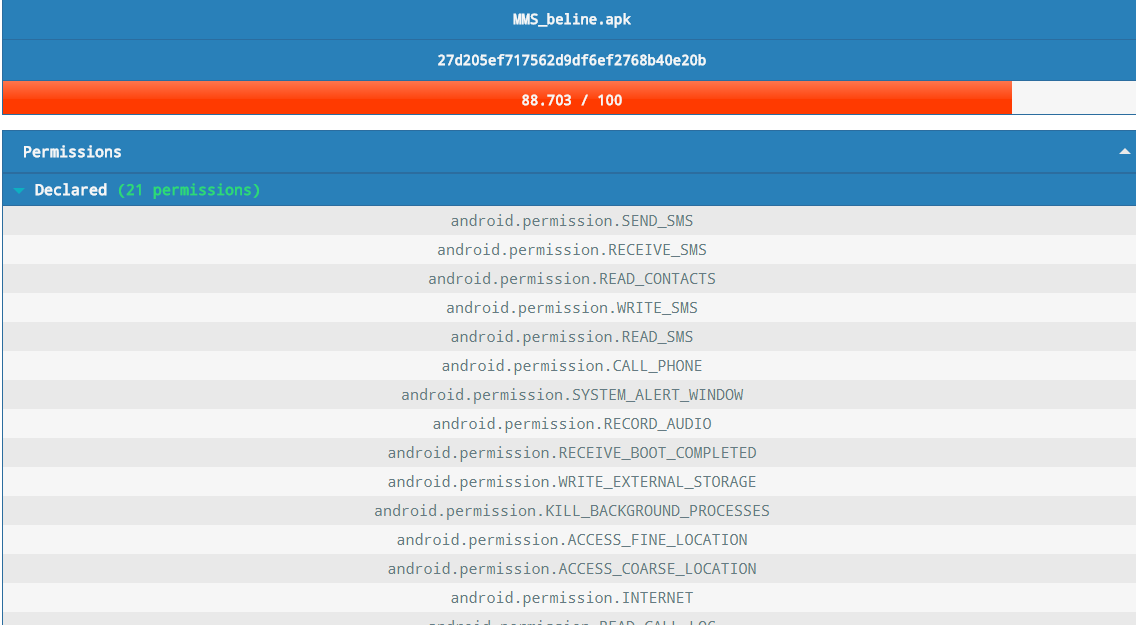
\includegraphics [scale=0.5] {mms.png}
  \caption{Screenshot captured during analysis of MMS Beline app}
  \label{fig:mms}
\end{figure}
\subsubsection{Permissions}
We have extracted the following permissions during the static analysis of MMS beline app:\\
\textbf{Required and used} (5 permissions)
\begin{itemize}
\begin{spacing}{0.9}
\item \texttt{android.permission.ACCESS\_FINE\_LOCATION} \hfill - Dangerous
\item \texttt{android.permission.ACCESS\_COARSE\_LOCATION} \hfill - Dangerous
\item \texttt{android.permission.INTERNET}
\item \texttt{android.permission.GET\_TASKS}
\item \texttt{android.permission.READ\_PHONE\_STATE} \hfill - Dangerous
\end{spacing}
\end{itemize}
\textbf{Required but not used} (16 permissions)
\begin{itemize}
\begin{spacing}{0.9}
\item \texttt{android.permission.SEND\_SMS} \hfill - Dangerous
\item \texttt{android.permission.RECEIVE\_SMS} \hfill - Dangerous
\item \texttt{android.permission.READ\_CONTACTS} \hfill - Dangerous
\item \texttt{android.permission.WRITE\_SMS} \hfill - Dangerous
\item \texttt{android.permission.READ\_SMS} \hfill - Dangerous
\item \texttt{android.permission.CALL\_PHONE} \hfill - Dangerous
\item \texttt{android.permission.SYSTEM\_ALERT\_WINDOW}
\item \texttt{android.permission.RECORD\_AUDIO} \hfill - Dangerous
\item \texttt{android.permission.RECEIVE\_BOOT\_COMPLETED}
\item \texttt{android.permission.WRITE\_EXTERNAL\_STORAGE} \hfill - Dangerous
\item \texttt{android.permission.KILL\_BACKGROUND\_PROCESSES} \hfill - Dangerous
\item \texttt{android.permission.READ\_CALL\_LOG} \hfill - Dangerous
\item \texttt{android.permission.ACCESS\_NETWORK\_STATE}
\item \texttt{android.permission.WAKE\_LOCK}
\item \texttt{android.permission.CAMERA} \hfill - Dangerous
\item \texttt{android.permission.READ\_EXTERNAL\_STORAGE} \hfill - Dangerous
\end{spacing}
\end{itemize}
\subsection{Google Calendar}
Google Calendar is the free time management web application offered by Google.Google Calendar allows users to create and edit events. Reminders can be enabled for events, with options available for type and time. Event locations can also be added, and other users can be invited to events. Users can enable or disable the visibility of special calendars, including Birthdays, where the app retrieves dates of births from Google contacts and displays birthday cards on a yearly basis, and Holidays, a country-specific calendar that displays dates of special occasions. Figure \ref{fig:cal} shows the screenshot taken during the static analysis of Calendar app.
\begin{figure}[!h]
  \centering
  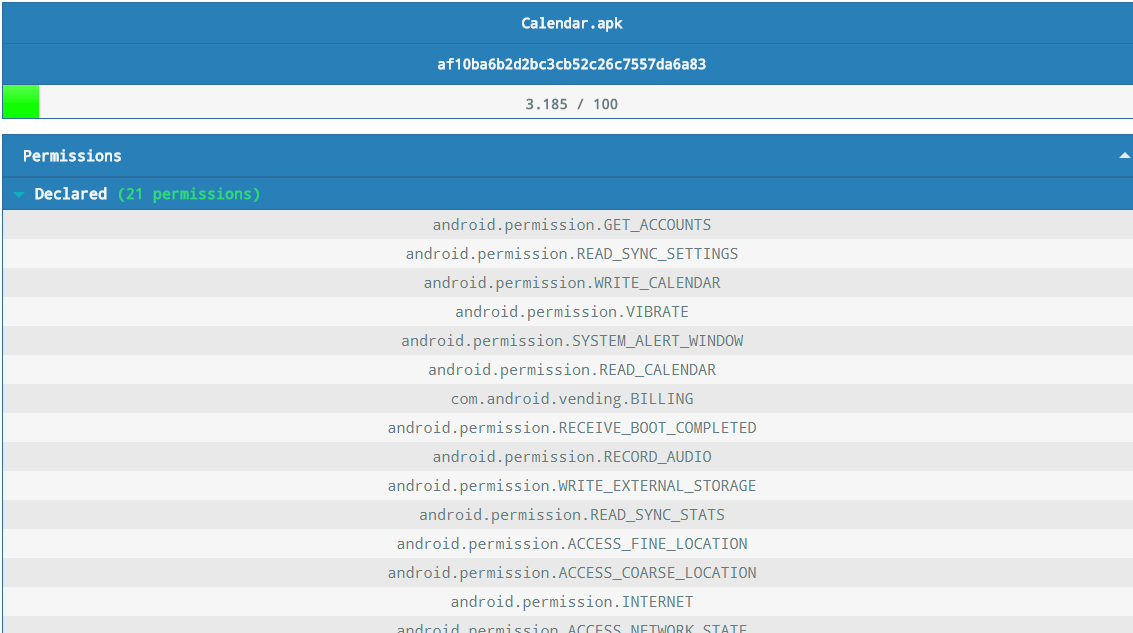
\includegraphics [scale=0.5] {cal.png}
  \caption{Screenshot captured during analysis}
  \label{fig:cal}
\end{figure}
\subsubsection{Permissions}
We have extracted the following permissions during the static analysis of Calendar app:\\
\textbf{Required and used} (8 permissions)
\begin{itemize}
\begin{spacing}{0.9}
\item \texttt{android.permission.ACCESS\_FINE\_LOCATION} \hfill - Dangerous
\item \texttt{android.permission.ACCESS\_COARSE\_LOCATION} \hfill - Dangerous
\item \texttt{android.permission.INTERNET}
\item \texttt{android.permission.VIBRATE}
\item \texttt{android.permission.ACCESS\_NETWORK\_STATE}
\item \texttt{android.permission.WAKE\_LOCK}
\item \texttt{android.permission.RECORD\_AUDIO} \hfill - Dangerous
\item \texttt{android.permission.WRITE\_EXTERNAL\_STORAGE} \hfill - Dangerous
\end{spacing}
\end{itemize}
\textbf{Required but not used} (13 permissions)
\begin{itemize}
\begin{spacing}{0.9}
\item \texttt{android.permission.GET\_ACCOUNTS} \hfill - Dangerous
\item \texttt{android.permission.READ\_SYNC\_SETTINGS}
\item \texttt{android.permission.WRITE\_CALENDAR} \hfill - Dangerous
\item \texttt{android.permission.SYSTEM\_ALERT\_WINDOW}
\item \texttt{android.permission.READ\_CALENDAR} \hfill - Dangerous
\item \texttt{com.android.vending.BILLING}
\item \texttt{android.permission.RECEIVE\_BOOT\_COMPLETED}
\item \texttt{android.permission.READ\_SYNC\_STATS}
\item \texttt{android.permission.GET\_TASKS}
\item \texttt{android.permission.READ\_EXTERNAL\_STORAGE} \hfill - Dangerous
\item \texttt{android.permission.WRITE\_SETTINGS}
\item \texttt{android.permission.READ\_PHONE\_STATE}
\item \texttt{com.google.android.providers.gsf.permission.READ\_GSERVICES}
\end{spacing}
\end{itemize}
\subsubsection{Unique Android SDK API methods}
Number of unique API calls count observed in the run is 4. Following is list of first calls to unique Android SDK API methods:
\begin{itemize}
    \item \texttt{0m 12s  - android.app.ActivityThread: void installContentProviders (android. content.Context, java.util.List)}
  \item \texttt{0m 12s  -  android.content.ContentResolver: android.database.Cursor query (android.net.Uri, java.lang.String[], java.lang.String, java.lang.String[], java.lang.String,android.os. CancellationSignal)}
 \item  \texttt{0m 12s  -  android.content.ContentResolver: android.database. Cursor query (android.net.Uri, java.lang.String[], java.lang.String,java.lang.String[],  java.lang.String, android.os. CancellationSignal)}
\item   \texttt{0m 12s  -  android.content.ContentResolver: android.database.Cursor query ( android.net.Uri, java.lang.String[], java.lang.String, java.lang.String[], java.lang.String,android.os. CancellationSignal)}
\item   \texttt{0m 12s  -  android.content.ContentResolver:void registerContentObserver( android.net.Uri, boolean ,android.database.ContentObserver, int)}
\item   \texttt{0m 12s -  android.content.ContentResolver: void registerContentObserver (android.net.Uri, boolean, android.database.ContentObserver, int)}
  \item \texttt{0m 12s  -  android.content.ContentResolver: android.database.Cursor query (android.net.Uri, java.lang.String[], java.lang.String, java.lang.String[], java.lang.String, android.os. CancellationSignal)}
 \item  \texttt{0m 12s  -  android.content.ContentResolver: android.database.Cursor query (android.net.Uri, java.lang.String[], java.lang.String, java.lang.String[],  java.lang.String,android.os. CancellationSignal)}
 \item  \texttt{0m 24s  -  android.content.ContentResolver: android.database.Cursor query (android.net.Uri, java.lang.String[], java.lang.String,java.lang.String[],  java.lang.String,android.os. CancellationSignal)}
 \item  \texttt{0m 27s  -  android.content.ContentResolver: android.database.Cursor query (android.net.Uri, java.lang.String[], java.lang.String,java.lang.String[], java.lang.String,android.os. CancellationSignal)}
 \item  \texttt{0m 31s  -  android.content.ContentResolver: android.database.Cursor query  (android.net.Uri, java.lang.String[], java. lang.String,java.lang.String[], j ava.lang.String,android.os. CancellationSignal)}
  \item \texttt{0m 33s  -  android.content.ContentResolver: android.database.Cursor query (android.net.Uri, java.lang.String[], java.lang.String, java.lang.String[], java.lang.String, android.os. CancellationSignal)}
 \item  \texttt{0m 38s  -  android.content.ContentResolver: android.database. Cursor query (android.net.Uri, java.lang.String[], java.lang.String, java.lang.String[],  java.lang.String,android. os.CancellationSignal)}
\item   \texttt{0m 38s  -  android.content.ContentResolver: void registerContentObserver (android.net.Uri, boolean, android.database.ContentObserver, int)}
 \item  \texttt{1m 21s  -  android.content.ContentResolver: android.database.Cursor query (android.net.Uri, java.lang.String[], java.lang.String, java.lang.String[], java.lang.String, android.os. CancellationSignal)}
 \item  \texttt{1m 23s  -  android.content.ContentResolver: android.database.Cursor query (android.net.Uri, java.lang.String[], java.lang.String, java.lang.String[], java.lang.String,android.os. CancellationSignal)}
 \item  \texttt{1m 54s  -  android.content.ContentResolver: android.database.Cursor query (android.net.Uri, java.lang.String[], java.lang.String, java.lang.String[], java.lang.String, android.os. CancellationSignal)}
 \item  \texttt{1m 56s  -  android.content.ContentResolver: android.database.Cursor query (android.net.Uri, java.lang.String[], java.lang.String, java.lang.String[], java.lang.String, android.os. CancellationSignal)}
 \item  \texttt{2m 11s   -  android.content.ContentResolver: android.database.Cursor query (android.net.Uri, java.lang.String[], java.lang.String, java.lang.String[],  java.lang.String, android.os. CancellationSignal)}

\end{itemize}

Figure \ref{fig:cal_api} shows the time at which different APIs and (API call, event) pairs are discovered. Total API discovered is 4 and total (API call,event) pair discovered is 5.
\begin{figure}[!h]
  \centering
  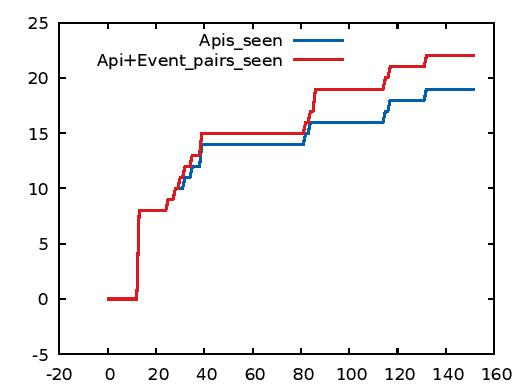
\includegraphics [scale=1.4] {cal_api.jpg}
  \caption{API count vs Exploration time}
  \label{fig:cal_api}
\end{figure}

\subsubsection{Actionable views}
According Figure \ref{fig:cal_view}, nearly 180 unique actionable views is seen and 33 out of 180 views are clicked. The Table \ref{table:2} shows 18 views are clicked once and 6 views are clicked twice. 
\begin{figure}[!h]
  \centering
  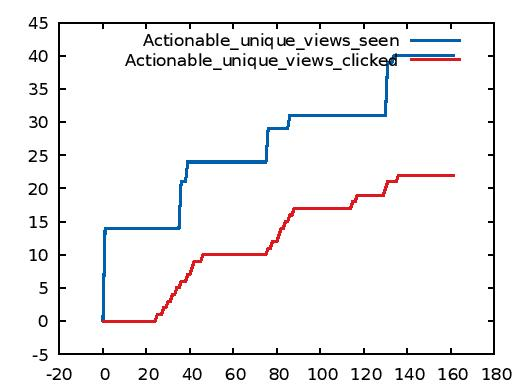
\includegraphics [scale=1.4] {cal_view.jpg}
  \caption{API count vs Exploration time}
  \label{fig:cal_view}
\end{figure}

\begin{table}[h!]
\centering
\begin{tabular}{||c | c||} 
 \hline
 Number of Click & Views Count \\ [0.5ex] 
 \hline\hline
 0 & 0 \\ 
 1 & 18\\
 2 & 6\\ [1ex] 

 \hline
\end{tabular}
\caption{Click Frequency of views}

\label{table:2}
\end{table}

\subsubsection{Aggregate stats}
Following is the summary of dynamic analysis of Google Calendar application:
\begin{itemize}
\begin{spacing}{1.2}
\item File name - Calendar-inlined.apk
\item Package name - com.google.android.calendar
\item Exploration seconds - 167
\item Actions - 35
\item In this reset actions - 4
\item Actionable unique views seen at least once - 40
\item Actionable unique views clicked or long clicked at least once - 22
\item Unique apis - 19
\item Unique event api pairs - 22
\item Exception - N/A (lack of DeviceException)
\end{spacing}
\end{itemize}

%---------------------------------------------------------------------%

%---------------------------------------------------------------------%


%---------------------------------------------------------------------%
%---------------------------------------------------------------------%
%------------------------------------------------------------------------------%
\subsection{Laughtter}
Laughtter is an application which can add charges to your mobile bill by sending costly SMS message without informing you first. Figure \ref{fig:laughtter} shows the screenshot taken during analysis of Laughtter app.
\begin{figure}[!h]
  \centering
  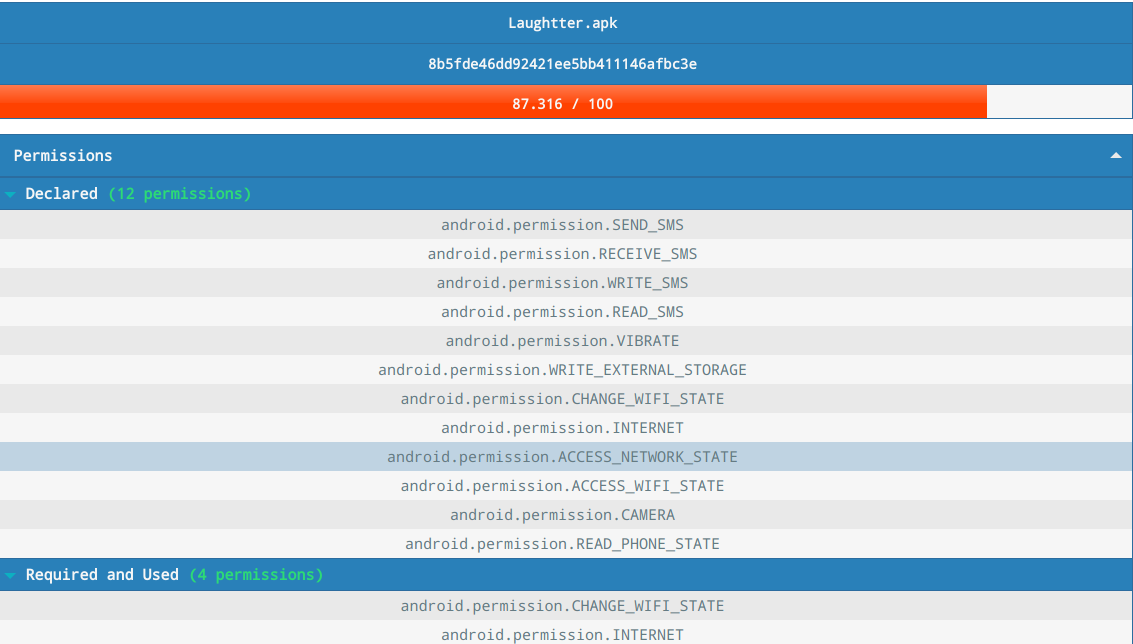
\includegraphics [scale=0.5] {laughtter.png}
  \caption{Screenshot captured during analysis of Laughtter app}
  \label{fig:laughtter}
\end{figure}
\subsubsection{Permissions}
We have extracted the following permissions during the static analysis of Laughtter app:\\
\textbf{Required and used} (4 permissions)
\begin{itemize}
\begin{spacing}{0.9}
\item \texttt{android.permission.CHANGE\_WIFI\_STATE}
\item \texttt{android.permission.INTERNET}
\item \texttt{android.permission.ACCESS\_NETWORK\_STATE}
\item \texttt{android.permission.ACCESS\_WIFI\_STATE}
\end{spacing}
\end{itemize}
\textbf{Required but not used} (8 permissions)
\begin{itemize}
\begin{spacing}{0.9}
\item \texttt{android.permission.SEND\_SMS} \hfill - Dangerous
\item \texttt{android.permission.RECEIVE\_SMS} \hfill - Dangerous
\item \texttt{android.permission.WRITE\_SMS} \hfill - Dangerous
\item \texttt{android.permission.READ\_SMS} \hfill - Dangerous
\item \texttt{android.permission.VIBRATE}
\item \texttt{android.permission.WRITE\_EXTERNAL\_STORAGE} \hfill - Dangerous
\item \texttt{android.permission.CAMERA} \hfill - Dangerous
\item \texttt{android.permission.READ\_PHONE\_STATE} \hfill - Dangerous
\end{spacing}
\end{itemize}
\textbf{Not required but used} (1 permissions)
\begin{itemize}
    \item \texttt{android.permission.WAKE\_LOCK}
\end{itemize}

\subsection{Android Framework}
Android Framework lets control your device, giving them unauthorized access to your data. Figure \ref{fig:andro} shows the screenshot taken during static analysis of the application.
\begin{figure}[!h]
  \centering
  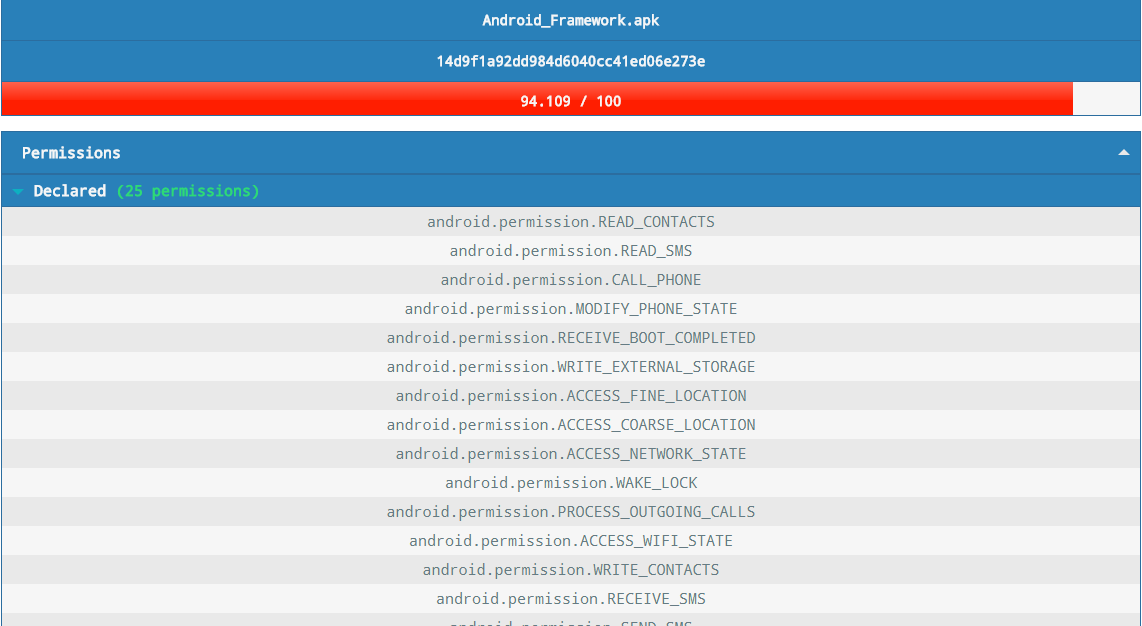
\includegraphics [scale=0.5] {andro.png}
  \caption{Screenshot captured during analysis of Android Framework app}
  \label{fig:andro}
\end{figure}
\subsubsection{Permissions}
We have extracted following permissions during the analysis of Android Framework application:\\
\textbf{Requested and used} (9 permissions)
\begin{itemize}
\begin{spacing}{0.9}    
\item \texttt{android.permission.ACCESS\_FINE\_LOCATION} \hfill - Dangerous
\item \texttt{android.permission.ACCESS\_COARSE\_LOCATION} \hfill - Dangerous
\item \texttt{android.permission.CHANGE\_WIFI\_STATE}
\item \texttt{android.permission.INTERNET}
\item \texttt{android.permission.ACCESS\_NETWORK\_STATE}
\item \texttt{android.permission.WAKE\_LOCK}
\item \texttt{android.permission.ACCESS\_WIFI\_STATE}
\item \texttt{android.permission.RECORD\_AUDIO} \hfill - Dangerous
\item \texttt{android.permission.READ\_PHONE\_STATE} \hfill - Dangerous
\end{spacing}
\end{itemize}
\textbf{Requested but not used} (16 permissions)
\begin{itemize}
\begin{spacing}{0.9}
\item \texttt{android.permission.READ\_CONTACTS} \hfill - Dangerous
\item \texttt{android.permission.READ\_SMS} \hfill - Dangerous
\item \texttt{android.permission.CALL\_PHONE} \hfill - Dangerous
\item \texttt{android.permission.MODIFY\_PHONE\_STATE} \hfill - Dangerous
\item \texttt{android.permission.RECEIVE\_BOOT\_COMPLETED}
\item \texttt{android.permission.WRITE\_EXTERNAL\_STORAGE} \hfill - Dangerous
\item \texttt{android.permission.PROCESS\_OUTGOING\_CALLS} \hfill - Dangerous
\item \texttt{android.permission.WRITE\_CONTACTS} \hfill - Dangerous
\item \texttt{android.permission.RECEIVE\_SMS} \hfill - Dangerous
\item \texttt{android.permission.SEND\_SMS} \hfill - Dangerous
\item \texttt{android.permission.WRITE\_APN\_SETTINGS}
\item \texttt{android.permission.WRITE\_SMS} \hfill - Dangerous
\item \texttt{android.permission.BROADCAST\_PACKAGE\_REMOVED}
\item \texttt{android.permission.CHANGE\_NETWORK\_STATE}
\item \texttt{android.permission.MODIFY\_AUDIO\_SETTINGS}
\item \texttt{android.permission.READ\_EXTERNAL\_STORAGE} \hfill - Dangerous
\end{spacing}
\end{itemize}


